\documentclass[tikz,border=12pt]{standalone}
\usetikzlibrary{calc, arrows.meta, positioning, decorations.markings}

\begin{document}
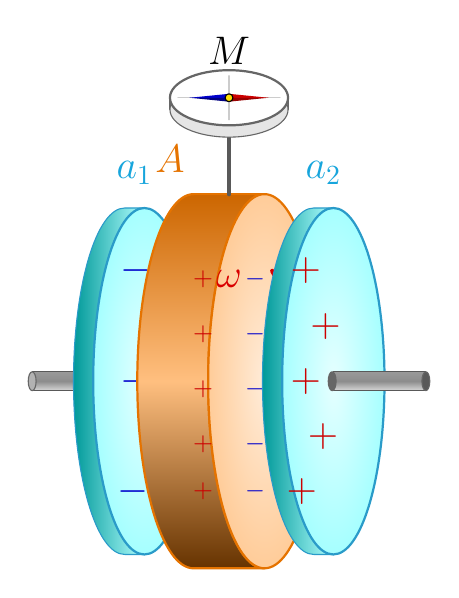
\begin{tikzpicture}[
    >=Stealth,
    line join=round,
    line cap=round,
    font=\sffamily
]

  % ==================== ПАРАМЕТРИ ====================
  \def\rx{0.65}     % Горизонтальний радіус дисків
  \def\ry{2.2}      % Вертикальний радіус дисків
  \def\tA{0.9}      % Товщина діелектрика A
  \def\ta{0.25}     % Товщина дисків a1, a2
  \def\rshaft{0.12} % Радіус вала

  \def\xA{0}        % Центр діелектрика A
  \def\xaOne{-1.2}  % Лівий диск a1
  \def\xaTwo{1.2}   % Правий диск a2
  \def\yM{3.6}      % Висота компаса M

  % ==================== 1. ВАЛ (ЛІВИЙ КРАЙ) ====================
  % Зовнішній лівий вал
  \shade[top color=gray!80, bottom color=gray!30, middle color=gray!90, draw=gray!70!black]
    (\xaOne-1.3, \rshaft) rectangle (\xaOne-\ta/2, -\rshaft);
  \filldraw[fill=gray!60, draw=gray!80!black] (\xaOne-1.3, 0) ellipse (0.05 and \rshaft);

  % ==================== 2. ЛІВИЙ ДИСК a1 (ОБКЛАДКА, -) ====================
  % Задня грань та бічниця
  \shade[left color=cyan!60!black, right color=cyan!30, draw=cyan!80!black]
    (\xaOne-\ta/2, \ry) arc (90:270:{\rx} and {\ry}) -- (\xaOne+\ta/2, -\ry) arc (270:90:{\rx} and {\ry}) -- cycle;
  % Передня грань
  \shade[inner color=cyan!10, outer color=cyan!35, draw=cyan!80!black, thick]
    (\xaOne+\ta/2, 0) ellipse ({\rx} and {\ry});

  % Заряди (-) на a1
  \foreach \y/\xoff in {1.4/-0.1, 0.7/0.15, 0.0/-0.1, -0.7/0.12, -1.4/-0.15}{
      \node[blue!80!black, font=\bfseries\Large] at (\xaOne+\ta/2+\xoff, \y) {$-$};
  }
  \node[cyan!90!black, font=\Large\bfseries] at (\xaOne, \ry+0.45) {$a_1$};

  % ==================== 3. ВАЛ (СЕРЕДИНА ЛІВА) ====================
  \shade[top color=gray!80, bottom color=gray!30, middle color=gray!90, draw=gray!70!black]
    (\xaOne+\ta/2, \rshaft) rectangle (\xA-\tA/2, -\rshaft);

  % ==================== 4. ЦЕНТРАЛЬНИЙ ДІЕЛЕКТРИК A ====================
  % Задня грань та бічна поверхня
  \shade[top color=orange!80!black, bottom color=orange!40!black, middle color=orange!50, draw=orange!90!black, thick]
    (\xA-\tA/2, \ry*1.08) arc (90:270:{\rx*1.1} and {\ry*1.08}) -- (\xA+\tA/2, -\ry*1.08) arc (270:90:{\rx*1.1} and {\ry*1.08}) -- cycle;
  % Передня грань
  \shade[inner color=orange!15, outer color=orange!40, draw=orange!90!black, thick]
    (\xA+\tA/2, 0) ellipse ({\rx*1.1} and {\ry*1.08});

  % Зв'язані поляризаційні заряди на гранях діелектрика
  \foreach \y in {1.3, 0.6, -0.1, -0.8, -1.4}{
      \node[red!80!black, font=\bfseries\small] at (\xA-\tA/2+0.12, \y) {$+$};
      \node[blue!80!black, font=\bfseries\small] at (\xA+\tA/2-0.12, \y) {$-$};
  }

  \node[orange!90!black, font=\Large\bfseries] at (\xA-\tA/2-0.3, \ry*1.08+0.45) {$A$};

  % Стрілка обертання \omega

  \draw[->, >=Stealth, red!85!black, ultra thick] 
    (\xA+\tA/2+0.1, 1.4) arc (60:-50:{\rx*0.9} and {\ry*0.75});
  \node[red!85!black, font=\Large] at (\xA, 1.3) {$\omega$};

  % ==================== 5. ВАЛ (СЕРЕДИНА ПРАВА) ====================
  \shade[top color=gray!80, bottom color=gray!30, middle color=gray!90, draw=gray!70!black]
    (\xA+\tA/2, \rshaft) rectangle (\xaTwo-\ta/2, -\rshaft);

  % ==================== 6. ПРАВИЙ ДИСК a2 (ОБКЛАДКА, +) ====================
  % Задня грань та бічниця
  \shade[left color=cyan!60!black, right color=cyan!30, draw=cyan!80!black]
    (\xaTwo-\ta/2, \ry) arc (90:270:{\rx} and {\ry}) -- (\xaTwo+\ta/2, -\ry) arc (270:90:{\rx} and {\ry}) -- cycle;
  % Передня грань
  \shade[inner color=cyan!10, outer color=cyan!35, draw=cyan!80!black, thick]
    (\xaTwo+\ta/2, 0) ellipse ({\rx} and {\ry});

  % Заряди (+) на a2
  \foreach \y/\xoff in {1.4/-0.1, 0.7/0.15, 0.0/-0.1, -0.7/0.12, -1.4/-0.15}{
      \node[red!80!black, font=\bfseries\Large] at (\xaTwo-\ta/2+\xoff, \y) {$+$};
  }
  \node[cyan!90!black, font=\Large\bfseries] at (\xaTwo, \ry+0.45) {$a_2$};

  % ==================== 7. ВАЛ (ПРАВИЙ КРАЙ) ====================
  \shade[top color=gray!80, bottom color=gray!30, middle color=gray!90, draw=gray!70!black]
    (\xaTwo+\ta/2, \rshaft) rectangle (\xaTwo+1.3, -\rshaft);
  \filldraw[fill=gray!70!black, draw=gray!80!black] (\xaTwo+1.3, 0) ellipse (0.05 and \rshaft);
  \filldraw[fill=gray!80!black, draw=gray!80!black] (\xaTwo+0.11, 0) ellipse (0.05 and \rshaft);

  % ==================== 8. МАГНІТНЕ ПОЛЕ B ====================
  % Силова лінія магнітного поля
%  \draw[teal!80!black, thick, dashed, postaction={decorate, decoration={markings, mark=at position 0.35 with {\arrow{Stealth[length=3mm]}}}}]
%    (\xA, 0) ellipse (1.35 and 3.4);
%  \node[teal!80!black, font=\bfseries\Large] at (\xA+1.65, 2.2) {$\vec{B}$};

  % ==================== 9. КОМПАС M МАЗУРИ ====================
  % Стійка
  \draw[gray!70!black, ultra thick] (\xA, \ry*1.08) -- (\xA, \yM-0.2);

  % Корпус компаса (3D дифузор)
  \shade[top color=gray!30, bottom color=gray!70, draw=gray!80!black]
    (\xA-0.75, \yM-0.15) rectangle (\xA+0.75, \yM);
  \filldraw[fill=gray!20, draw=gray!80!black] (\xA, \yM-0.15) ellipse (0.75 and 0.35);
  \filldraw[fill=white, draw=gray!80!black, thick] (\xA, \yM) ellipse (0.75 and 0.35);

  % Шкала компаса
  \draw[gray!40, thin] (\xA-0.65, \yM) -- (\xA+0.65, \yM);
  \draw[gray!40, thin] (\xA, \yM-0.28) -- (\xA, \yM+0.28);

  % Об'ємна 3D стрілка компаса
  % Північний полюс (червоний, вправо)
  \fill[red!80!black] (\xA, \yM+0.05) -- (\xA+0.5, \yM) -- (\xA, \yM) -- cycle;
  \fill[red!60!black] (\xA, \yM-0.05) -- (\xA+0.5, \yM) -- (\xA, \yM) -- cycle;
  % Південний полюс (синій, вліво)
  \fill[blue!80!black] (\xA, \yM+0.05) -- (\xA-0.5, \yM) -- (\xA, \yM) -- cycle;
  \fill[blue!50!black] (\xA, \yM-0.05) -- (\xA-0.5, \yM) -- (\xA, \yM) -- cycle;

  % Центр стрілки (заклепка)
  \filldraw[fill=yellow!80!orange, draw=black, thin] (\xA, \yM) circle (0.05);

  \node[font=\Large\bfseries] at (\xA, \yM+0.6) {$M$};

\end{tikzpicture}
\end{document}